\section{Численный расчёт для системы волновод\,--\,массив нанодисков}

При расчётах массива нанодисков использовался метод последовательных приближений: зная оптимальную конфигурацию для $n$ дисков, оптимальное решение для системы из $n+1$ дисков искалось как изначальная система с варьирующимся расстоянием между дисками номер $n$ и $n+1$. Собственные параметры резонаторов были зафиксированы на оптимальных значениях, представленных в таблице \ref{tbl:effective_params}.

Помимо глубины резонансного провала для потенциального создания оптического переключателя также важна его ''острота``, то есть максимальная производная. Глубина провала считалась как разница между минимальным значением и средним от левого и правого края резонанса. Максимальная производная искалась на левой стороне пика, как на более устойчивой к изменению количества резонаторов. Эти два показателя и были основной метрикой, по которой производилась оптимизация конфигурации из нескольких нанодисков.

Для устранения краевых эффектов между крайними дисками и торцами волновода всегда оставлялся зазор длиной не менее 1 мкм. Так как в пространство у одной стороны волновода длиной 10 мкм эффективно умещается 15 нанодисков, то было решено попробовать исследовать конфигурацию, в которой диски находятся с обеих сторон волновода. Моделирование показало, что оптимальной конфигурацией является размещение дисков одной стороны в промежутках между дисками второй стороны.

Ввиду большого количества графиков (более 400) спектров пропускания волновода в зависимости от расстояния между дисками, ограничимся сводными зависимостями глубины пика (рис. \ref{fig:metrics_dT}) и его максимальной производной (рис. \ref{fig:metrics_dTdLambda}), а также графиками спектров (рис. \ref{fig:Nx_fixed_r_fixed_d}) для наиболее удачных значений расстояния между дисками для каждого из количеств резонаторов.

\begin{figure}[h]
	\begin{subfigure}[b]{.5\textwidth}
		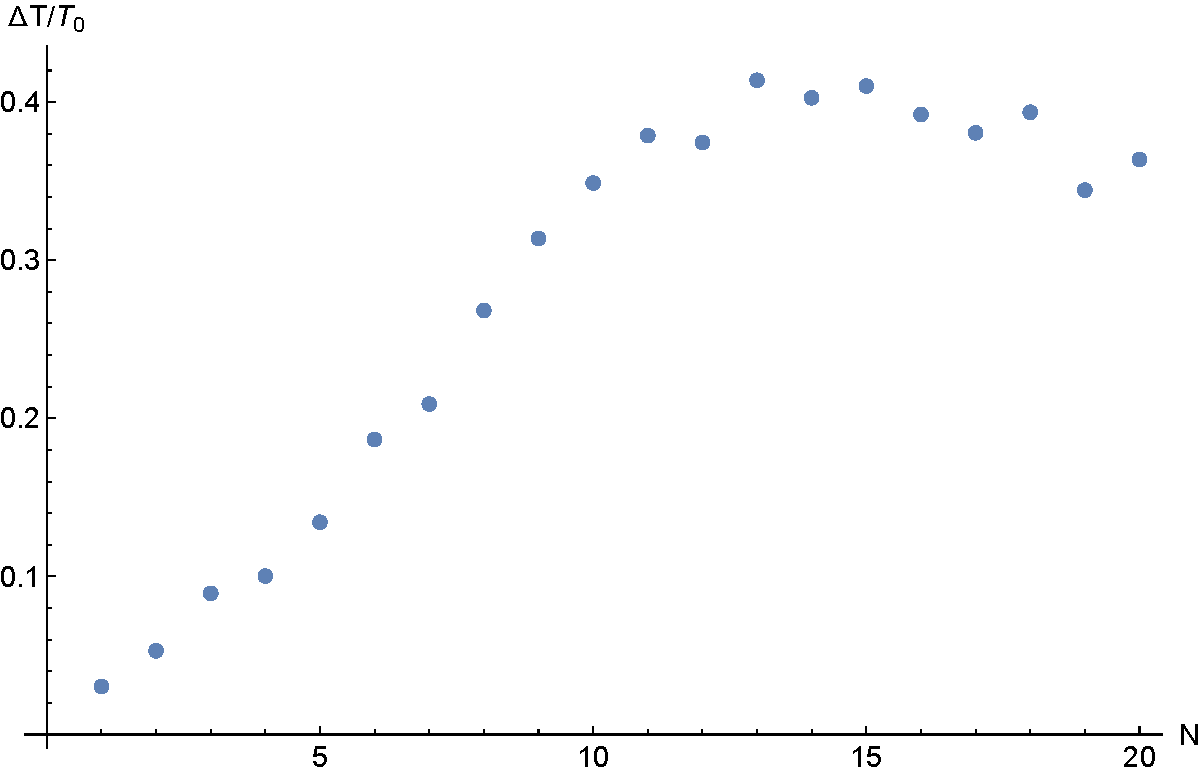
\includegraphics[width=\textwidth]{img/dTPlot}
		\caption{Глубина пика}
		\label{fig:metrics_dT}
	\end{subfigure}
	\begin{subfigure}[b]{.5\textwidth}
		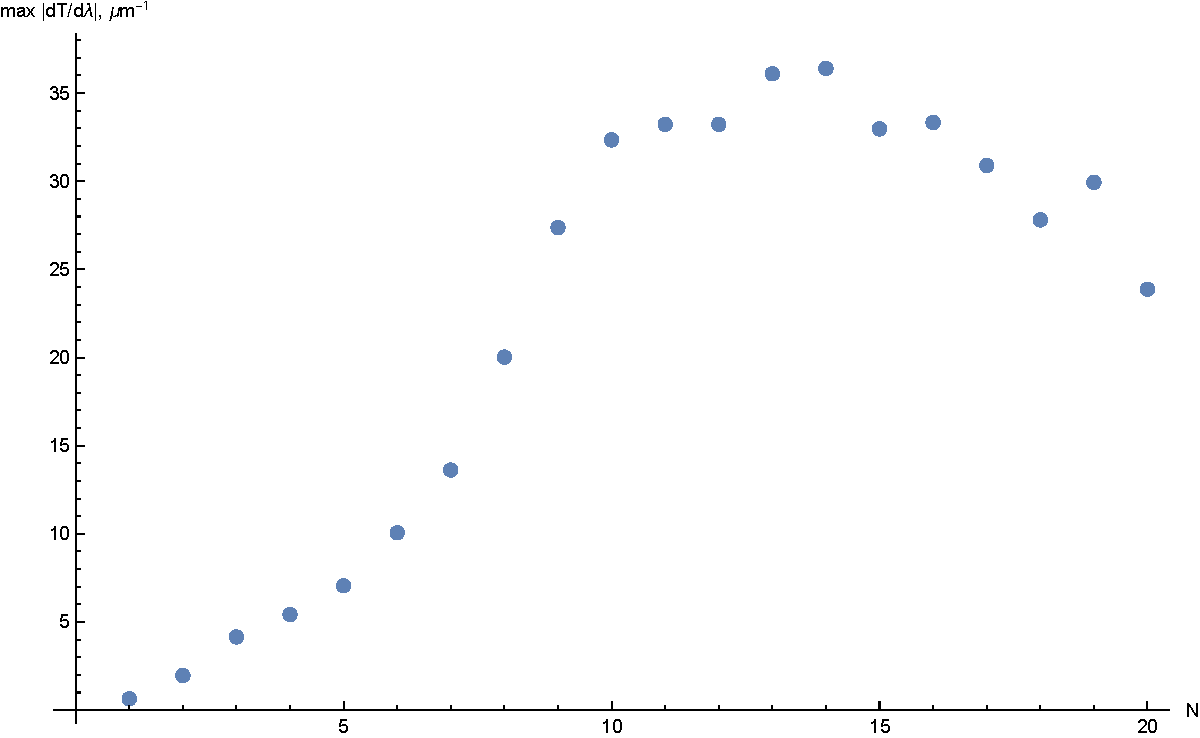
\includegraphics[width=\textwidth]{img/dTdλPlot}
		\caption{''Острота`` резонанса}
		\label{fig:metrics_dTdLambda}
	\end{subfigure}
	\caption{Сводные графики основных метрик}
	\label{fig:metrics}
\end{figure}

\begin{figure}[h]
	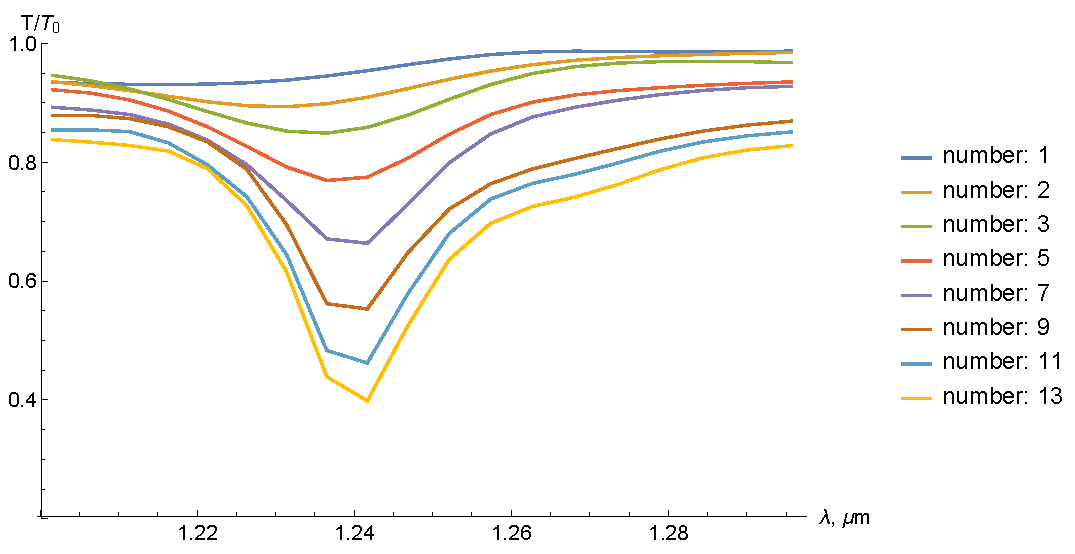
\includegraphics[width=\textwidth]{img/total}
	\caption{Спектр пропускания волновода в зависимости от количества нанодисков}
	\label{fig:Nx_fixed_r_fixed_d}
\end{figure}

Из вида зависимости метрик от количества связанных с волноводом резонаторов (рис. \ref{fig:metrics}) можно заключить, что максимальная эффективность достигается массивом из 13 нанодисков. Вид такой системы показан на рисунке \ref{fig:scheme_final_13}, а координаты дисков указаны в таблице \ref{tbl:x_coords}. Порядковый номер диска и его X-координата отсчитываются от левого торца волновода.

\begin{figure}[h]
	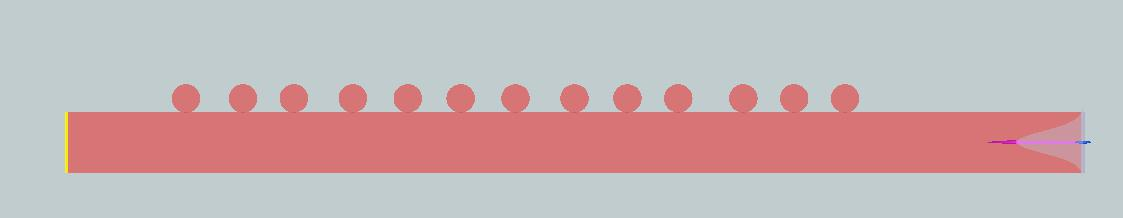
\includegraphics[width=\textwidth]{img/view_xy_13}
	\caption{Рассчитанная конфигурация из 13 нанодисков}
	\label{fig:scheme_final_13}
\end{figure}

\begin{table}[h]
	\centering
	\begin{tabular}{|c|c|c|c|c|c|c|}
		\hline
		N & 1 & 2 & 3 & 4 & 5 & 6 \\
		\hline
		x, мкм & 1.18 & 1.74 & 2.24 & 2.82 & 3.36 & 3.88 \\
		\hline
		\hline
		7 & 8 & 9 & 10 & 11 & 12 & 13 \\
		\hline
		4.42 & 5.00 & 5.52 & 6.02 & 6.66 & 7.16 & 7.66 \\
		\hline
	\end{tabular}
	\caption{X-координаты нанодисков в наиболее эффективной конфигурации}
	\label{tbl:x_coords}
\end{table}